\documentclass[conference,10pt]{IEEEtran}
\usepackage[utf8]{inputenc}
\usepackage{times}
\usepackage{graphicx}
\usepackage{booktabs}
\usepackage{amsmath}
\usepackage{url}
\usepackage[hidelinks]{hyperref}
\usepackage{xcolor}
\usepackage{tikz}
\usetikzlibrary{arrows.meta,positioning,shapes.geometric}
\usepackage{longtable}
\usepackage{listings}
\lstset{basicstyle=\ttfamily\footnotesize,breaklines=true,columns=fullflexible}

\newcommand{\code}[1]{\texttt{\small #1}}

\begin{document}

\title{A Reproducible Study of Client-Side Request Signing on Two Social Platforms: Virtualization versus Obfuscation}

\author{\IEEEauthorblockN{Sreenandhu Nair}
\IEEEauthorblockA{Independent security research\\
\texttt{https://github.com/zkp6c4vr89-coder/tiktok-xhs-signing-analysis}}}

\maketitle

\begin{abstract}
Large web platforms attach cryptographic-looking signatures to API requests to tell real browsers from automated clients. We study the client-side signing code of two of them, TikTok (the \code{webmssdk} script that emits \code{X-Bogus} and \code{X-Gnarly}) and Xiaohongshu / RedNote (the \code{x-s} header), as a reproducibility exercise. We independently replicate a prior community analysis of TikTok's bytecode virtual machine against a current bundle, and apply the same toolkit to Xiaohongshu. Our contribution is understanding and reusable tooling, not a means of access: no working signer is released. We find that the two platforms make opposite architectural choices. TikTok virtualizes its signer into a bespoke register machine (we recover \textbf{365} opcodes and \textbf{351} functions and disassemble \textbf{89.7\%} of a 98{,}961-byte bytecode image), whereas Xiaohongshu ships string-array- and control-flow-obfuscated JavaScript over two encrypted data blobs. We also document that TikTok \emph{replaced} its VM between the version a 2025 analysis examined (core 1.12.2) and the one we captured (1.16.6): stack machine to register machine, 77 to 365 opcodes. In both cases a runtime environment-integrity check, not the obfuscation, was the barrier to end-to-end extraction; we stopped at that boundary by design. Every number in this paper traces to a script, trace, or data file in the public repository.
\end{abstract}

\section{Introduction}
Modern social platforms protect their web APIs by having the browser compute a signature over each request and send it in custom headers. A request without a valid signature is rejected, so the signing code is a high-value target for both scrapers and defenders. The code ships to every visitor, so it is heavily obfuscated.

This paper treats two such systems as objects of a \emph{reproducibility} study. Part~A independently replicates a 2025 community reverse-engineering of TikTok's \code{webmssdk}~\cite{tiktokref} against a bundle we captured ourselves. Part~B applies the resulting toolkit to Xiaohongshu's \code{x-s} signature. Part~C compares them. The guiding constraint is that the contribution is \emph{understanding plus reusable analysis tooling}, never a usable signer: we publish algorithm descriptions, diagrams, test vectors, and pass/fail results, and we keep raw bundles and any validation-only reimplementation out of the public repository.

\noindent\textbf{Contributions.}
\begin{itemize}
  \item An independent, reproducible replication of the TikTok \code{webmssdk} VM analysis against a current bundle, with a reusable bytecode decoder, opcode-table builder, and disassembler (Section~\ref{sec:tiktok}).
  \item A finding that TikTok \emph{replaced} its protection VM between versions (stack to register machine, 77 to 365 opcodes, 272 to 351 functions), making a prior static analysis obsolete (Sections~\ref{sec:tiktok},~\ref{sec:compare}).
  \item The first (to our knowledge) write-up of the current Xiaohongshu \code{x-s} signer's structure: a \code{javascript-obfuscator} payload over two encrypted data blobs, with the input/output contract and a reusable evaluating deobfuscation pass (Section~\ref{sec:xhs}).
  \item A comparative taxonomy of the two defensive strategies, and the observation that in both cases a runtime integrity check, not the code obfuscation, was the true analysis barrier (Section~\ref{sec:compare}).
  \item A fully reproducible pipeline (\code{make reproduce}) and an explicit ethical boundary: we decline to defeat the integrity checks because that crosses into building a signer (Section~\ref{sec:ethics}).
\end{itemize}

\section{Background and Related Work}
\label{sec:background}
\textbf{JavaScript obfuscation and deobfuscation.} Obfuscation hides a program's intent while preserving behaviour; Collberg \emph{et al.}~\cite{collberg1997taxonomy} give the classic taxonomy (layout, data, and control transformations, judged by potency, resilience, stealth, and cost). On the web specifically, Skolka \emph{et al.}~\cite{skolka2019anything} measured obfuscation in the wild and found that most obfuscated scripts resemble the output of a single tool and that such code is disproportionately used for fingerprinting---both borne out by our Xiaohongshu case.

\textbf{Virtualization-based obfuscation.} The strongest technique we encounter translates logic into bytecode for a custom interpreter. Rolles~\cite{rolles2009unpacking} framed these obfuscators as interpreters that can be attacked by writing a disassembler for their bytecode; Sharif \emph{et al.}~\cite{sharif2009emulators} automated reverse-engineering of such emulators dynamically; Yadegari \emph{et al.}~\cite{yadegari2015generic} gave a semantics-based, obfuscation-agnostic deobfuscator. Our TikTok work is a hand-built instance of Rolles's recipe applied to a JavaScript VM.

\textbf{Fingerprinting and bot detection.} Signing is one half of bot detection; the other is binding the signature to hard-to-forge device state. Eckersley~\cite{eckersley2010unique} showed browser configurations are widely unique; Nikiforakis \emph{et al.}~\cite{nikiforakis2013cookieless} dissected commercial fingerprinting providers; Laperdrix \emph{et al.}~\cite{laperdrix2020fingerprinting} survey the area. The environment reads we record (Section~\ref{sec:compare}) are exactly the surface these works describe.

\textbf{Prior work on these platforms.} The TikTok analysis we replicate is a community repository~\cite{tiktokref}; the author describes it as a rapid effort and invites correction. Xiaohongshu's \code{x-s} has been discussed in blog posts and the open-source \emph{xhshow} project; we treat those as leads to verify, not ground truth, and we did not consult \emph{xhshow}'s source during our own analysis.

\section{Ethics and Scope}
\label{sec:ethics}
This is defensive and educational research with no affiliation to either company. We observe four rules. (1)~\emph{No signer is released.} The public repository contains descriptions, diagrams, test vectors, and pass/fail results; any reimplementation built to validate understanding stays in a git-ignored directory and is never published. (2)~\emph{We work offline.} The live sites were touched only to capture public static bundles, logged out, at human pace, with a generic user agent and no cookies; no automated or bulk requests were sent to any API. When a CDN returned HTTP~403 without a site referer, we declined to spoof headers to retrieve the file. (3)~\emph{No personal data.} All harness inputs are synthetic; no real accounts, cookies, or device identifiers appear anywhere. (4)~\emph{No full bundles.} We publish only SHA-256 hashes, URLs, capture dates, and the short excerpts needed to make a point; the copyrighted bundles stay git-ignored.

A consequence worth stating plainly: both signers abort when run outside a real browser because of a runtime \emph{environment-integrity check}. Defeating that check is the step that would turn our understanding into a working signer, so \emph{we deliberately stop there}. This is a scope boundary, not a failed attempt; it is why Section~\ref{sec:xhs} reports no valid \code{x-s} test vectors.

\section{Methodology}
\label{sec:method}
All analysis runs offline against pinned bundles. Each analysed file is recorded in \code{data/bundles.csv} with platform, filename, URL, SHA-256, and capture date, and \code{make verify-samples} checks every local sample against its hash. The offline pipeline (\code{make reproduce}) runs deobfuscation, disassembly, tracing, and figure generation from the pinned inputs.

The toolkit is written to be reused across both platforms. \emph{Deobfuscation} (\code{tools/deobf/}) uses Babel to parse each bundle into an AST and apply passes: a classic string-array pass that resolves \code{ARR[n]} and decoder-call indirections to literals, and an evaluating pass that handles the \code{javascript-obfuscator} preset by running the array/rotation/decoder prelude in a sandboxed \code{node:vm} context and rewriting decoder calls with their decoded values. \emph{Virtual-machine analysis} (\code{tools/vm/}) comprises a bytecode loader, an opcode-table builder that extracts the handler array and classifies each handler's operand encoding on the AST, a linear and recursive-descent disassembler, and a string-pool decoder. \emph{Tracing} (\code{tools/harness/}) runs the signer in a \code{node:vm} context whose global is a logging-Proxy browser shim.

The shim is the same for both platforms. Every property read on \code{window}, \code{navigator}, \code{document}, \code{screen}, and their descendants is recorded through nested \code{Proxy} objects, producing the fingerprint surface. All values are fixed synthetic stubs, and \code{Date} and \code{Math.random} are made deterministic, so a trace is reproducible and contains no personal data. We inject two hooks into the bundle source before running it: one on the VM's string decoder (to log every decoded string with its key) and one on the dispatch site (to count executed opcodes). Every quantitative claim below is produced by one of these tools and is regenerable with \code{make reproduce}.

\section{Case Study 1: TikTok}
\label{sec:tiktok}
\textbf{Bundle.} The reference analysis~\cite{tiktokref} pinned no hash; it pasted deobfuscated source, from which we recovered the version it examined: \code{webmssdk} core \textbf{1.12.2}. A logged-out load of \code{tiktok.com} referenced one signer URL, from which we captured \code{webmssdk} core \textbf{1.16.6} (asset \code{1.0.0.417}; SHA-256 \code{6625c4fd{\ldots}}). The four-minor-version gap is the study's first finding.

\textbf{Strings.} The reference removed a JavaScript-level string array with a Babel \code{MemberExpression} pass. In 1.16.6 that layer is \emph{gone}: no rotating string array, zero \code{parseInt} checksums, no 40-element string-literal arrays. The strings moved into the VM bytecode, decoded at runtime by a base64-plus-repeating-XOR routine. Our reusable string-array pass therefore has no target here---a concrete instance of version drift changing the obfuscation surface.

\textbf{The VM.} 1.16.6 is a \emph{register} machine, not the reference's stack machine (Fig.~\ref{fig:arch}). The interpreter function \code{S(start,this,args,ctx,\_,L)} builds a frame \code{u} with a register file \code{u.o} (slots 0--6 preloaded with \code{null}, \code{undefined}, \code{true}, \code{false}, a return sentinel, the arguments, and the call context), a program counter \code{u.I} into the decompressed bytecode, a try/handler stack \code{u.A}, and a boundary \code{u.L} above which registers are boxed closure cells. The dispatch loop is
\begin{lstlisting}
while (u.I < g.length && C(u,4) === w) {
  f = (g[u.I++]<<8) | g[u.I++];   // 16-bit opcode
  d[f](u);                        // handler
}
return C(u,4);                    // write reg 4 = return
\end{lstlisting}
Each handler reads its operands with three readers (\code{O} for 1 byte, \code{p} for 2 bytes, \code{m} for 3 bytes) and accesses registers through getters/setters (\code{C}/\code{L} get, \code{Q}/\code{I} set). A function returns by writing register~4, which ends the loop. Table~\ref{tab:vm} summarises these elements.

Bytecode is delivered as base64 then raw DEFLATE, the decompression the reference had hard-coded around, yielding a 98{,}961-byte image. We implement the loader (\code{tools/vm/decode.js}), extract the handler table (\textbf{365} opcodes; Fig.~\ref{fig:opcats}), classify each handler's operand encoding on the AST, and build a recursive-descent disassembler. Function entries come from 206 constant \code{S(\ldots)} offsets plus operand-driven children; following them reaches \textbf{351} functions, \textbf{245} of which return cleanly, covering \textbf{89.7\%} of the image (Fig.~\ref{fig:coverage}). The entry function disassembles as, e.g.:
\begin{lstlisting}
  0  op218 store        [0, 14, 8]
  7  op175 make-function [52,46,9,10,24,54]
 23  op148 make-function [9,56,14,868,11]
 36  op353 call          [1,1,10,1,4,7,11]
\end{lstlisting}
Many opcodes are specialised: 99 are \emph{terminal} (each inlines a whole function body and ends with a write to register~4), which is why 365 exceeds the reference's 77---the compiler emitted one handler per operation shape rather than a fixed instruction set. The count 365 is exact (the handler-array length); the category breakdown in Fig.~\ref{fig:opcats} is a heuristic labelling of handler bodies and is not load-bearing for any count.

\begin{figure}[t]
  \centering
  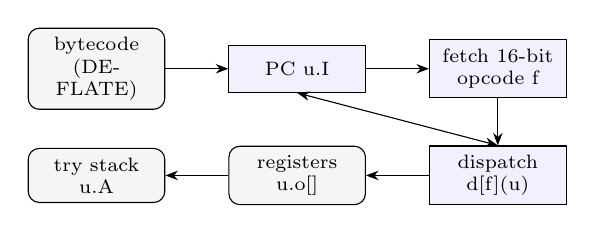
\begin{tikzpicture}[
    node distance=4mm and 8mm,
    reg/.style={draw,rounded corners,align=center,font=\scriptsize,text width=15mm,minimum height=6mm,fill=black!4},
    op/.style={draw,align=center,font=\scriptsize,text width=15mm,minimum height=6mm,fill=blue!6},
    >={Stealth[length=1.6mm]}]
    \node[reg] (bc) {bytecode (DEFLATE)};
    \node[op,right=of bc] (pc) {PC u.I};
    \node[op,right=of pc] (fetch) {fetch 16-bit opcode f};
    \node[op,below=6mm of fetch] (disp) {dispatch d[f](u)};
    \node[reg,left=of disp] (regs) {registers u.o[]};
    \node[reg,left=of regs] (astk) {try stack u.A};
    \draw[->] (bc)--(pc); \draw[->] (pc)--(fetch); \draw[->] (fetch)--(disp);
    \draw[->] (disp)--(regs); \draw[<->] (disp.north)--(pc.south);
    \draw[->] (regs)--(astk);
  \end{tikzpicture}
  \caption{TikTok \code{webmssdk} 1.16.6 register-VM architecture: a 16-bit opcode is fetched from the DEFLATE-decompressed bytecode and dispatched through a 365-entry handler table that reads operands and mutates the register file; writing register 4 returns.}
  \label{fig:arch}
\end{figure}

\begin{table}[t]
\caption{1.16.6 VM state and primitives (recovered in \code{tools/vm/}).}
\label{tab:vm}
\centering\footnotesize
\begin{tabular}{@{}ll@{}}
\toprule
Element & Role \\
\midrule
\code{u.o[]} & register file (0--6 preloaded) \\
\code{u.I} & program counter (byte offset) \\
\code{u.A} & try/exception handler stack \\
\code{u.L} & boxed-register boundary \\
\code{O/p/m} & 1/2/3-byte operand readers \\
\code{C,L} / \code{Q,I} & register get / set \\
write \code{u.o[4]} & function return \\
\code{l(n,t)} & string decode: base64 then XOR key $t$ \\
\bottomrule
\end{tabular}
\end{table}

\begin{figure}[t]
  \centering
  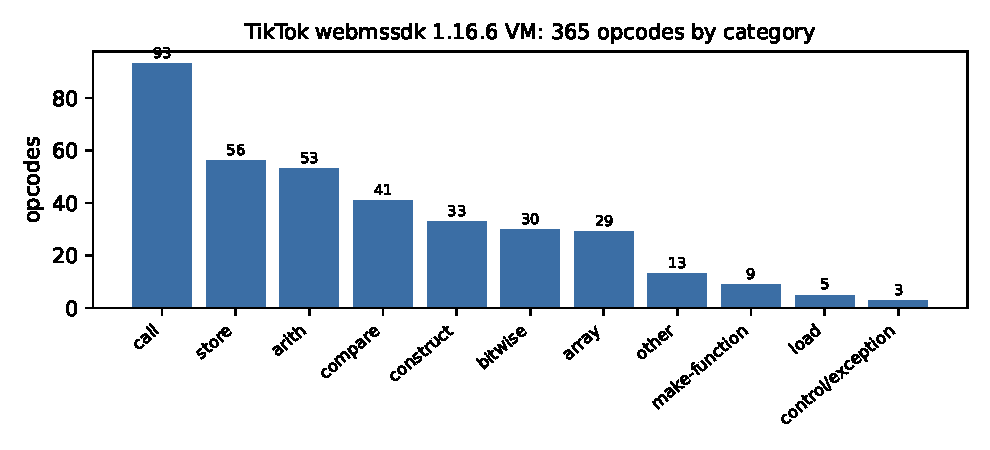
\includegraphics[width=\columnwidth]{figures/fig_opcode_categories.pdf}
  \caption{Opcode categories recovered from the TikTok \code{webmssdk} 1.16.6 handler table (365 opcodes), generated by \code{make\_figures.py} from \code{data/tiktok\_opcodes\_1.16.6.json}.}
  \label{fig:opcats}
\end{figure}

\begin{figure}[t]
  \centering
  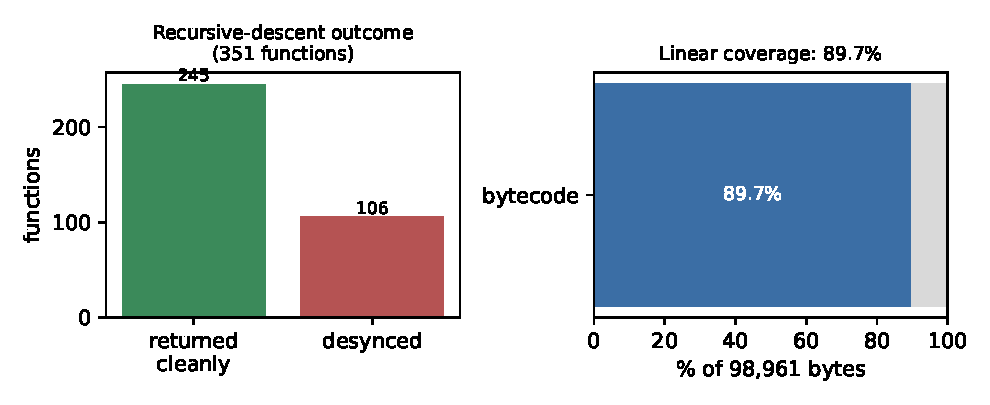
\includegraphics[width=\columnwidth]{figures/fig_coverage.pdf}
  \caption{Recursive-descent disassembly outcome and linear byte coverage for the 1.16.6 bytecode image.}
  \label{fig:coverage}
\end{figure}

\textbf{Tracing.} Under the harness, the bootstrap executes 8{,}884 VM dispatches across 89 opcodes before it halts on environment APIs we do not emulate; the decoder hook recovers correct plaintext, confirming the string model. We recover the token names from the base64/XOR pool by keeping only exact matches (an exact ``\code{X-Bogus}'' decode cannot be coincidental): \code{X-Bogus} at pool index~686, \code{X-Gnarly} at~688, \code{msToken} at~685. Scanning the disassembly for instructions that load those indices maps each token to its producing functions---\code{X-Bogus} at \code{fn@70647} and neighbours, \code{X-Gnarly} at \code{fn@73223}, all assembled at \code{fn@61636}. This is our analog of the reference's \code{vm103}/\code{vm249} result; the offsets differ because the VM differs. The numeric constant pool names the primitives: an LCG increment, the golden-ratio constant \code{0x9E3779B9}, SHA-256 round constants, FNV offsets, and the \code{strData} envelope magic \code{538969122}; a bundled MD5 (\code{JS\_MD5\_NO\_NODE\_JS}) appears in the fingerprint surface. We did not produce a signature headless, so the exact composition is stated as referenced, not byte-confirmed.

\textbf{Worked example: from bytecode bytes to \code{X-Bogus}.} To make the pipeline concrete, we trace one instruction end to end. In \code{fn@61636} (the header-assembly function), byte offset 62{,}053 holds
\begin{lstlisting}
01 20  02 ae  00 05  00 07  00 1b
\end{lstlisting}
The dispatcher reads the first two bytes as the opcode \code{0x0120 = 288} (an array-build handler) and then four 2-byte operands: \code{0x02ae = 686}, 5, 7, 27. Operand 686 is a string-pool index. Pool entry \code{A[686]} is the base64 string \code{"PVgnJSUPHg=="}; decoding it (base64, then XOR with the pooled key \code{A[5] = "eueJBzmo"}) yields exactly \code{"X-Bogus"}. So this instruction, in this function, places the \code{X-Bogus} header name into an array under construction---which is how we attribute the token to \code{fn@61636} without executing it. The same chain recovers \code{X-Gnarly} (\code{A[688]}) and \code{msToken} (\code{A[685]}). Every step here is reproduced by \code{tools/vm/disasm.js} and \code{tools/vm/strings.js}.

Table~\ref{tab:replication} is the claim-by-claim replication (full detail in \code{analysis/tiktok/REPLICATION.md}). Of 12 claims, 5 reproduce directly, 5 reproduce in a different form attributable to the version change, 1 is a technique with no target in 1.16.6, and 1 (exact end-to-end composition) is unverified. No claim contradicted the reference outright; the divergences are all explained by the VM replacement.

\begin{table}[t]
\caption{TikTok claim-by-claim replication. R~=~reproduced; R$^\ast$~=~reproduced in a different form (version drift); T~=~technique only; U~=~unverified.}
\label{tab:replication}
\centering\footnotesize
\resizebox{\columnwidth}{!}{%
\begin{tabular}{@{}p{0.62\columnwidth}l@{}}
\toprule
Reference claim & Verdict \\
\midrule
A bytecode VM protects the signer & R \\
VM is a \emph{stack} machine with a \code{switch} & R$^\ast$ (register, handler table) \\
77 opcodes & R$^\ast$ (365) \\
272 VM functions & R$^\ast$ (351 found) \\
JS-level string array (Babel-removable) & T (absent in 1.16.6) \\
Varint bytecode parser, no decompression & R$^\ast$ (base64+DEFLATE) \\
Per-function disassembly & R \\
Custom runtime string decoder & R (base64+XOR) \\
\code{vm103}/\code{vm249}=X-Bogus/X-Gnarly & R$^\ast$ (\code{fn@70647}/\code{fn@73223}) \\
MD5 in the pipeline & R (MD5 lib flag) \\
Mixing with \code{0x9E3779B9} & R (pool constant) \\
Exact X-Bogus byte composition & U \\
\bottomrule
\end{tabular}}
\end{table}

\section{Case Study 2: Xiaohongshu}
\label{sec:xhs}
\textbf{Contract.} \code{xiaohongshu.com} redirects to the \code{rednote.com} rebrand, whose login page still serves the public PC-web bundles. The signer lives in \code{vendor-dynamic} (SHA-256 \code{25e31f6b{\ldots}}). An axios interceptor establishes the contract: \code{l = window.sign(url, body)} returns a header object merged into the request, carrying \code{x-s}, \code{x-t}, and \code{x-s-common}; \code{\_webmsxyw} is the newer signer global. Inputs are the request URL (URI plus serialized query), the body, the \code{a1} cookie (with \code{webId}/\code{gid}), and a timestamp (Fig.~\ref{fig:pipelines}).

\textbf{Form and deobfuscation.} The signer is embedded as a 288{,}347-character string that the bundle \code{eval}s. It begins \code{var \_0x5ae8=[\ldots]}---a \code{javascript-obfuscator} string array of 1045 entries, with a decoder (\code{\_0xc8b2}), an alias (\code{\_0xe762c0}), and a rotation IIFE that reorders the array under a \code{parseInt} checksum:
\begin{lstlisting}
var _0x5ae8=['doeZk','vSuEv',...];      // pool
var _0xc8b2=function(i,k){...            // decoder
  ...return _0x5ae8[i-0x0]...};
var _0xe762c0=_0xc8b2;                   // alias
(function(a,b){while(!![]){...           // rotation
  a['push'](a['shift']());...}}(_0x5ae8,0x1a2));
glb[_0xe762c0(0x73)]=function(a,b,c){...} // signer
\end{lstlisting}
We built an evaluating string-array pass (\code{tools/deobf/passes/string-array-eval.js}) that detects the decoder structurally, resolves its aliases transitively (40 here, including per-function local aliases), evaluates the array/rotation/decoder prelude in a sandbox, and rewrites literal-argument calls. It resolves 297 of them; e.g.\ \code{glb[\_0xe762c0(0x73)]} becomes \code{glb["\_AUuXfEG27Xa3x"]}. Three layers remain: computed-index decoder calls, control-flow flattening (\code{while(true)\{switch\}} dispatchers), and two encrypted hex data blobs (\code{\_\_\$c}, \code{\_\_bc}) that the signer interprets---so the signer is partly data-driven, not pure inline JavaScript. This is still far more readable than TikTok's VM: roughly 90\% is ordinary JS after the pass, versus 0\% before the VM is rebuilt.

\textbf{Algorithm (partial) and vectors.} Under the harness the payload loads and defines the signer \code{glb["\_AUuXfEG27Xa3x"](url,body,ctx)}, but it aborts with an environment-integrity error after reading \code{document.documentElement.getAttribute}. A reachable helper builds a to-be-signed string of the form \code{url + 1013904243}---the same LCG constant seen in TikTok. Primitive evidence is partial: base64 (\code{atob}) is confirmed; MD5 is referenced but its magic constants are not plaintext (they live in the encrypted blobs), so MD5 use is \emph{referenced, not byte-confirmed}; the older public claim of RC4 and a custom Base64/Base58 alphabet is \emph{not independently confirmed} on this 2026 bundle. Because the signer aborts, \textbf{we produced no valid \code{x-s} test vectors}; \code{data/test\_vectors/xhs.json} records the inputs, the integrity-check blocker, and a clearly-labelled non-signature partial output. The pass rate is therefore N/A by design (Section~\ref{sec:ethics}).

\begin{figure*}[t]
  \centering
  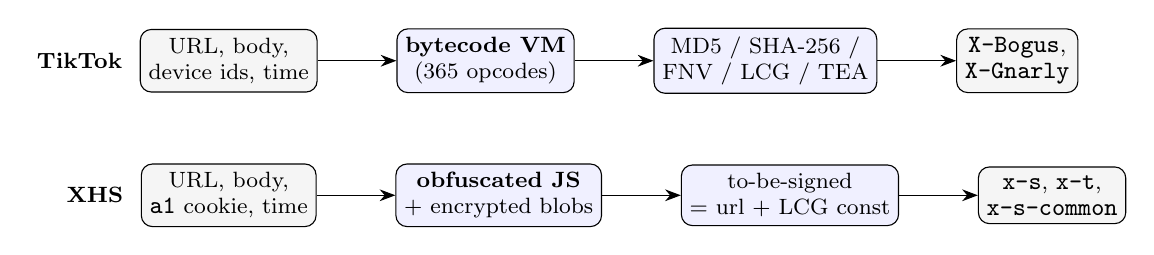
\begin{tikzpicture}[
    node distance=6mm and 10mm,
    box/.style={draw,rounded corners,align=center,font=\footnotesize,minimum height=7mm,inner sep=3pt},
    prim/.style={box,fill=blue!6},
    io/.style={box,fill=black!4},
    >={Stealth[length=2mm]}]
    % TikTok row
    \node[io] (ti) {URL, body,\\device ids, time};
    \node[prim,right=of ti] (tvm) {\textbf{bytecode VM}\\(365 opcodes)};
    \node[prim,right=of tvm] (tp) {MD5 / SHA-256 /\\FNV / LCG / TEA};
    \node[io,right=of tp] (to) {\code{X-Bogus},\\\code{X-Gnarly}};
    \draw[->] (ti)--(tvm); \draw[->] (tvm)--(tp); \draw[->] (tp)--(to);
    \node[left=1mm of ti,font=\footnotesize\bfseries] {TikTok};
    % XHS row
    \node[io,below=9mm of ti] (xi) {URL, body,\\\code{a1} cookie, time};
    \node[prim,right=of xi] (xo) {\textbf{obfuscated JS}\\+ encrypted blobs};
    \node[prim,right=of xo] (xp) {to-be-signed\\$=$ url $+$ LCG const};
    \node[io,right=of xp] (xout) {\code{x-s}, \code{x-t},\\\code{x-s-common}};
    \draw[->] (xi)--(xo); \draw[->] (xo)--(xp); \draw[->] (xp)--(xout);
    \node[left=1mm of xi,font=\footnotesize\bfseries] {XHS};
  \end{tikzpicture}
  \caption{The two signing pipelines at the level our evidence supports. Primitives shown for TikTok are named by its constant pool (referenced, not all byte-confirmed); the Xiaohongshu crypto core is partly inside encrypted data blobs we did not fully reverse.}
  \label{fig:pipelines}
\end{figure*}

\section{Comparative Analysis}
\label{sec:compare}
Table~\ref{tab:taxonomy} is the technique taxonomy. The headline is a choice of \emph{where to put the cost}. TikTok virtualizes: nothing is readable until the interpreter is rebuilt, but then coverage is broad. Xiaohongshu obfuscates ordinary JavaScript: most is readable after a string pass, but a small encrypted core resists. Both bind URL, body, a persistent identifier, and a millisecond timestamp into the signature, and both share a Numerical-Recipes LCG increment (\code{1013904223}/\code{1013904243}).

\begin{table}[t]
\caption{Obfuscation technique taxonomy. ``conf.''~=~confirmed by our tooling; ``ref.''~=~referenced in code/constants but not byte-confirmed.}
\label{tab:taxonomy}
\centering\footnotesize
\resizebox{\columnwidth}{!}{%
\begin{tabular}{@{}lll@{}}
\toprule
 & TikTok 1.16.6 & Xiaohongshu 2026 \\
\midrule
Core strategy & bytecode VM (conf.) & string array + CFG (conf.) \\
Dispatch & 365-opcode reg.\ VM & \code{while/switch} flattening \\
String hiding & base64+XOR pool (conf.) & array decoder+aliases (conf.) \\
Code/data packing & base64+DEFLATE (conf.) & encrypted blobs (conf.) \\
Hash primitives & MD5/SHA-256 (ref.) & MD5 (ref.), base64 (conf.) \\
Randomness & LCG, \code{0x9E3779B9} (conf.) & LCG const (conf.) \\
Anti-tamper & env init gate (conf.) & integrity check (conf.) \\
\bottomrule
\end{tabular}}
\end{table}

\textbf{Version drift.} For TikTok this is quantified: between core 1.12.2 and 1.16.6 the VM was replaced wholesale (stack~$\to$~register, 77~$\to$~365 opcodes, 272~$\to$~351 functions, JS string array~$\to$~in-VM pool, hard-coded bytes~$\to$~base64+DEFLATE). For Xiaohongshu we pinned a single bundle and make no cadence claim; we note only the rebrand and a modern obfuscator toolchain.

\textbf{Analysis difficulty.} We did not log wall-clock hours, so we report relative effort by tooling built: TikTok required five new tools (decoder, table builder, disassembler, pool decoder, harness) and was $\sim$0\% readable without them; Xiaohongshu required three and was $\sim$90\% readable after the string pass. TikTok has a higher up-front cost but broad payoff; Xiaohongshu is faster to first insight but its crypto core is gated.

\textbf{Lessons for defenders.} First, virtualization and obfuscation are a cost-shape choice, not a security level; both were analysable to the level needed to describe the pipeline. Second, and most important, \emph{the real barrier was the runtime environment-integrity check, not the code hiding}: binding signatures to hard-to-forge environment state stopped end-to-end extraction more cheaply than heavy static obfuscation. Third, well-known constants (LCG increments, \code{0x9E3779B9}, SHA-256 and MD5 tables) leak the primitive inventory before any deobfuscation. Fourth, version drift was the strongest defence we measured: TikTok's wholesale VM swap would break any static signer.

\section{Discussion and Limitations}
\label{sec:discussion}
Our results are bounded in ways we state explicitly. We produced no signature for either platform, so token-to-function maps come from static operand analysis, not from observing a live signature, and exact byte-level composition is unverified. Primitive claims marked ``referenced'' (notably MD5 on both platforms, and RC4/custom-alphabet on Xiaohongshu) are named in code or constants but not confirmed by reproducing an output. Fingerprint surfaces are the bootstrap-phase subset each signer reads before aborting, not the complete set. The TikTok disassembler does not yet follow the 33 in-function jump opcodes, so 106 of 351 functions desync and coverage is 89.7\%, not 100\%. Opcode categories are heuristic labels. For Xiaohongshu the encrypted \code{\_\_\$c}/\code{\_\_bc} blobs and control-flow flattening are not fully stripped. Finally, the 1.12.2 bundle the reference used is no longer served, so our cross-version comparison for TikTok relies partly on its pasted source. Several of these gaps (jump-aware disassembly, CFG unflattening) are tractable future work; others (defeating the integrity checks) are deliberately out of scope.

\section{Conclusion}
\label{sec:conclusion}
Two platforms, the same goal, opposite strategies: TikTok virtualizes its request signer into a 365-opcode register machine that it rotates aggressively across versions, while Xiaohongshu obfuscates ordinary JavaScript over an encrypted data core. We replicated the TikTok analysis against a current bundle, showed its VM had been replaced since the prior study, and produced a reusable offline toolkit that applies to both. In both cases the decisive defence was a runtime environment-integrity check rather than the obfuscation itself---a boundary we chose not to cross, which is precisely why no signer accompanies this paper.

\appendices
\section{Pinned Bundles}
All in \code{data/bundles.csv}, captured 2026-11-12/13, logged out, with SHA-256 pinned and checked by \code{make verify-samples}:
\begin{itemize}\footnotesize
  \item TikTok \code{webmssdk.1.0.0.417.js} (core 1.16.6), \code{6625c4fd{\ldots}a814c8}.
  \item Xiaohongshu \code{vendor-dynamic.bb0b0051.js} (signer), \code{25e31f6b{\ldots}}.
  \item Xiaohongshu \code{index}, \code{vendor}, \code{bundler-runtime} (siblings).
\end{itemize}

\section{Opcode Encoding (representative)}
Each row of \code{data/tiktok\_opcodes\_1.16.6.json} gives an opcode's operand-read sequence (hence its byte length), whether it writes the return register, and a heuristic category. Table~\ref{tab:opcodes} shows representative rows.

\begin{table}[h]
\caption{Representative opcodes (of 365). Reads: \code{O}=1B, \code{p}=2B, \code{m}=3B.}
\label{tab:opcodes}
\centering\footnotesize
\begin{tabular}{@{}rllrc@{}}
\toprule
op & category & reads & operand B & terminal \\
\midrule
0 & construct & -- & 0 & yes \\
1 & bitwise & -- & 0 & yes \\
2 & make-function & \code{ppm} & 7 & no \\
3 & call & \code{pppppp} & 12 & no \\
41 & compare & \code{ppmp} & 9 & no \\
65 & arith & \code{pppppp} & 12 & no \\
218 & store & \code{Opp} & 5 & no \\
347 & construct & \code{ppOppp} & 11 & no \\
\bottomrule
\end{tabular}
\end{table}

\section{Fingerprint Surfaces}
Both are the subset read before each signer aborts (Section~\ref{sec:discussion}).

\noindent\textbf{TikTok} (\code{data/tiktok\_fingerprint\_surface.json}):
\begin{itemize}\footnotesize\setlength\itemsep{0pt}
  \item \code{navigator}, \code{navigator.connection}
  \item \code{document.readyState}, \code{document.addEventListener}
  \item the Slardar telemetry registry
  \item a bundled MD5 flag (\code{JS\_MD5\_NO\_NODE\_JS})
\end{itemize}

\noindent\textbf{Xiaohongshu} (\code{data/xhs\_fingerprint\_surface.json}):
\begin{itemize}\footnotesize\setlength\itemsep{0pt}
  \item \code{document.cookie}
  \item \code{document.documentElement\allowbreak.getAttribute}
  \item \code{document.addEventListener}
\end{itemize}

\section{Pass and Tool Catalogue}
\code{tools/deobf/}: string-array pass and evaluating string-array pass (6 unit tests). \code{tools/vm/}: \code{decode.js}, \code{build\_opcode\_table.js}, \code{disasm.js}, \code{strings.js}, \code{pipeline.js} (3 tests). \code{tools/harness/}: \code{env.js} logging shim, \code{run\_tiktok.js}, \code{run\_xhs.js}. Token map in \code{data/tiktok\_token\_map\_1.16.6.json}; vectors status in \code{data/test\_vectors/xhs.json}.

\section{Full Opcode Table}
All 365 opcodes of the 1.16.6 VM, auto-generated from \code{data/tiktok\_opcodes\_1.16.6.json} by \code{paper/figures/make\_opcode\_table.py}. Columns per entry: opcode (\code{op}), heuristic category (\code{cat}: con/bit/mkf/cal/arr/sto/cmp/ari/lod/oth/ctl), and operand-read string (\code{rd}: \code{O}=1B, \code{p}=2B, \code{m}=3B; \code{--}=none).
\onecolumn
% AUTO-GENERATED by paper/figures/make_opcode_table.py -- do not edit by hand.
\begin{center}\footnotesize
\begin{longtable}{rll|rll|rll|rll}
op & cat & rd & op & cat & rd & op & cat & rd & op & cat & rd \\ \hline
\endhead
0 & con & -- & 1 & bit & -- & 2 & mkf & ppm & 3 & cal & pppppp \\
4 & arr & ppppp & 5 & sto & ppppp & 6 & bit & ppppp & 7 & cmp & pppppp \\
8 & con & ppppp & 9 & ari & ppppp & 10 & cmp & Oppp & 11 & mkf & -- \\
12 & cal & ppppppp & 13 & lod & ppppp & 14 & sto & p & 15 & cmp & -- \\
16 & cal & pppppp & 17 & sto & ppOp & 18 & ari & pp & 19 & ari & ppppp \\
20 & mkf & -- & 21 & sto & ppp & 22 & arr & pppp & 23 & cal & ppppppppp \\
24 & ari & ppppp & 25 & ari & pppppp & 26 & con & Opppp & 27 & ari & pppppp \\
28 & cal & -- & 29 & ari & ppp & 30 & cal & ppp & 31 & ari & -- \\
32 & cal & -- & 33 & cal & -- & 34 & cal & pppppppp & 35 & sto & p \\
36 & cal & -- & 37 & sto & pppp & 38 & cal & -- & 39 & ari & pppppp \\
40 & arr & ppppp & 41 & cmp & ppmp & 42 & oth & -- & 43 & cmp & ppppp \\
44 & arr & -- & 45 & cal & -- & 46 & sto & mpp & 47 & cal & ppppmmp \\
48 & arr & -- & 49 & cal & -- & 50 & sto & pp & 51 & cmp & mppp \\
52 & con & -- & 53 & cal & -- & 54 & con & ppppp & 55 & cmp & OpppO \\
56 & bit & pppppp & 57 & arr & pppp & 58 & cal & ppppppp & 59 & ari & pppppp \\
60 & sto & p & 61 & cal & -- & 62 & sto & ppppp & 63 & cal & -- \\
64 & cmp & ppp & 65 & ari & pppppp & 66 & bit & ppppp & 67 & cal & -- \\
68 & cal & -- & 69 & oth & -- & 70 & arr & pppppppp & 71 & lod & ppppppp \\
72 & cal & -- & 73 & cal & ppppppp & 74 & sto & -- & 75 & cal & ppppppp \\
76 & cmp & Opppp & 77 & bit & pppppp & 78 & cal & pppppppp & 79 & cmp & ppppp \\
80 & sto & ppp & 81 & arr & ppppp & 82 & bit & ppppp & 83 & cal & -- \\
84 & con & -- & 85 & cmp & Opmp & 86 & arr & pppp & 87 & oth & -- \\
88 & sto & -- & 89 & cmp & ppp & 90 & sto & ppp & 91 & bit & -- \\
92 & bit & -- & 93 & cal & pppppppppp & 94 & ctl & m & 95 & con & ppppp \\
96 & bit & ppp & 97 & sto & ppppppp & 98 & sto & pp & 99 & ari & pppppp \\
100 & mkf & mpOpp & 101 & ari & pppppp & 102 & ari & ppp & 103 & arr & pp \\
104 & bit & ppp & 105 & cal & ppppppppp & 106 & arr & -- & 107 & sto & OpOp \\
108 & lod & p & 109 & sto & pp & 110 & cmp & pp & 111 & bit & -- \\
112 & cal & pppppp & 113 & cal & ppppppp & 114 & arr & ppp & 115 & con & pppppp \\
116 & sto & Oppp & 117 & sto & pOOp & 118 & ari & pppppp & 119 & cal & ppppm \\
120 & cmp & pppppp & 121 & sto & pp & 122 & bit & ppp & 123 & cmp & ppp \\
124 & oth & m & 125 & cmp & pppmpm & 126 & bit & -- & 127 & cal & -- \\
128 & arr & -- & 129 & bit & ppppppp & 130 & cmp & pppm & 131 & cal & ppppppp \\
132 & cal & pppp & 133 & cmp & ppppp & 134 & sto & pppppp & 135 & cal & ppppppp \\
136 & bit & -- & 137 & cal & pppppppp & 138 & bit & mppp & 139 & cal & ppm \\
140 & cal & -- & 141 & con & ppppp & 142 & cal & pppppppp & 143 & cal & pppppppp \\
144 & cal & -- & 145 & con & -- & 146 & con & ppp & 147 & cal & -- \\
148 & mkf & pmppp & 149 & arr & ppppp & 150 & ari & ppppp & 151 & cmp & ppppp \\
152 & bit & pppppp & 153 & ari & ppppp & 154 & ari & ppp & 155 & cal & -- \\
156 & cal & ppppmm & 157 & mkf & mpppOp & 158 & oth & -- & 159 & cmp & pmpmpp \\
160 & ari & pppppp & 161 & cal & pppppp & 162 & arr & -- & 163 & cal & ppppppp \\
164 & ari & pppppp & 165 & ari & pppppp & 166 & cal & -- & 167 & bit & pppppp \\
168 & cmp & mppp & 169 & ari & ppp & 170 & ctl & -- & 171 & cal & -- \\
172 & ari & pppppp & 173 & sto & mp & 174 & arr & p & 175 & mkf & mppppm \\
176 & sto & pppp & 177 & oth & -- & 178 & lod & mpm & 179 & cal & pppppppppp \\
180 & cal & -- & 181 & con & -- & 182 & con & pppp & 183 & sto & pp \\
184 & arr & -- & 185 & cal & -- & 186 & cal & -- & 187 & sto & pp \\
188 & con & ppppppp & 189 & bit & pppppp & 190 & con & -- & 191 & sto & pppp \\
192 & oth & -- & 193 & ari & pppppp & 194 & cmp & ppp & 195 & ari & -- \\
196 & cmp & mpppmp & 197 & cmp & pmpmpp & 198 & cal & ppppppp & 199 & oth & -- \\
200 & sto & ppp & 201 & cmp & -- & 202 & ari & pppppppp & 203 & cal & -- \\
204 & bit & ppppp & 205 & con & pppppp & 206 & cal & ppppppppp & 207 & ari & ppppppp \\
208 & ari & -- & 209 & con & ppp & 210 & arr & pmpp & 211 & sto & ppppppp \\
212 & arr & ppppppp & 213 & sto & pp & 214 & sto & OpOp & 215 & sto & mmppp \\
216 & cmp & ppp & 217 & con & pppppp & 218 & sto & Opp & 219 & ari & -- \\
220 & cmp & ppppp & 221 & cmp & mpppmp & 222 & bit & -- & 223 & sto & ppmppm \\
224 & cal & ppppppppp & 225 & cal & -- & 226 & bit & ppppp & 227 & cal & pppppp \\
228 & cal & ppppppp & 229 & con & -- & 230 & cal & -- & 231 & ari & ppppp \\
232 & sto & ppm & 233 & sto & pppp & 234 & cal & -- & 235 & ari & pppp \\
236 & cmp & ppppp & 237 & con & -- & 238 & cal & -- & 239 & cal & pppppppppp \\
240 & bit & ppp & 241 & con & pppp & 242 & oth & -- & 243 & sto & ppp \\
244 & sto & ppppp & 245 & cal & pppp & 246 & con & -- & 247 & cmp & ppmp \\
248 & ari & pppppppppp & 249 & ari & pppppppppp & 250 & arr & pppppp & 251 & bit & pppppp \\
252 & con & -- & 253 & arr & pppppp & 254 & con & -- & 255 & cmp & pppOOp \\
256 & ari & pp & 257 & cal & pppp & 258 & cal & pppppp & 259 & cal & ppmppp \\
260 & cal & -- & 261 & oth & -- & 262 & cal & ppppppp & 263 & con & pppppp \\
264 & cmp & Opp & 265 & cal & -- & 266 & ari & -- & 267 & cal & ppppp \\
268 & cal & ppppppp & 269 & cal & -- & 270 & ari & ppOpp & 271 & mkf & pmppO \\
272 & ari & ppp & 273 & arr & ppppp & 274 & arr & pp & 275 & sto & pO \\
276 & con & pppppp & 277 & bit & -- & 278 & cal & ppppppppp & 279 & cmp & ppp \\
280 & cmp & ppmppm & 281 & oth & -- & 282 & ari & -- & 283 & cal & ppppp \\
284 & cmp & pOpOp & 285 & arr & pppp & 286 & ari & -- & 287 & ari & pmpp \\
288 & arr & pppp & 289 & sto & mpp & 290 & cal & -- & 291 & ari & pppppp \\
292 & sto & mpppp & 293 & bit & ppppp & 294 & sto & pp & 295 & ari & pppppp \\
296 & oth & -- & 297 & ari & ppp & 298 & ari & -- & 299 & con & -- \\
300 & arr & ppppppp & 301 & oth & -- & 302 & con & -- & 303 & cmp & pppppp \\
304 & sto & pp & 305 & cmp & pmpmpp & 306 & cal & -- & 307 & cmp & ppp \\
308 & arr & -- & 309 & cal & -- & 310 & cal & -- & 311 & sto & pO \\
312 & cal & -- & 313 & cal & mppp & 314 & cal & ppppppp & 315 & ari & pppppp \\
316 & bit & ppp & 317 & con & pppppp & 318 & bit & ppp & 319 & bit & ppppp \\
320 & sto & ppmp & 321 & ari & ppm & 322 & arr & p & 323 & ari & pppppp \\
324 & con & pppppp & 325 & cal & pppppppp & 326 & mkf & -- & 327 & sto & mmppp \\
328 & sto & pOp & 329 & cal & pppppp & 330 & cal & -- & 331 & cal & ppppppppppp \\
332 & cmp & -- & 333 & ari & pppppppp & 334 & sto & ppp & 335 & sto & ppppp \\
336 & cal & pppppppp & 337 & cmp & pppppp & 338 & cal & -- & 339 & cal & pppppppp \\
340 & sto & pppppp & 341 & sto & pppp & 342 & ctl & -- & 343 & ari & pppppp \\
344 & sto & ppp & 345 & bit & -- & 346 & sto & -- & 347 & con & ppOppp \\
348 & ari & pOpppp & 349 & con & -- & 350 & ari & ppppp & 351 & sto & pp \\
352 & cmp & ppp & 353 & cal & ppppppp & 354 & sto & pppp & 355 & arr & ppp \\
356 & ari & ppppppp & 357 & ari & -- & 358 & con & -- & 359 & cal & pppppppppp \\
360 & sto & ppppp & 361 & lod & ppp & 362 & cal & -- & 363 & cal & ppppp \\
364 & cal & -- &  & &  &  & &  &  & &  \\
\end{longtable}
\end{center}


\begin{thebibliography}{10}
\bibitem{collberg1997taxonomy} C.~Collberg, C.~Thomborson, and D.~Low, ``A Taxonomy of Obfuscating Transformations,'' Univ.\ of Auckland, Tech.\ Rep.\ 148, 1997.
\bibitem{skolka2019anything} P.~Skolka, C.-A.~Staicu, and M.~Pradel, ``Anything to Hide? Studying Minified and Obfuscated Code in the Web,'' in \emph{WWW}, 2019, pp.\ 1735--1746.
\bibitem{rolles2009unpacking} R.~Rolles, ``Unpacking Virtualization Obfuscators,'' in \emph{USENIX WOOT}, 2009.
\bibitem{sharif2009emulators} M.~Sharif, A.~Lanzi, J.~Giffin, and W.~Lee, ``Automatic Reverse Engineering of Malware Emulators,'' in \emph{IEEE S\&P}, 2009, pp.\ 94--109.
\bibitem{yadegari2015generic} B.~Yadegari, B.~Johannesmeyer, B.~Whitely, and S.~Debray, ``A Generic Approach to Automatic Deobfuscation of Executable Code,'' in \emph{IEEE S\&P}, 2015, pp.\ 674--691.
\bibitem{eckersley2010unique} P.~Eckersley, ``How Unique Is Your Web Browser?'' in \emph{PETS}, 2010, pp.\ 1--18.
\bibitem{nikiforakis2013cookieless} N.~Nikiforakis, A.~Kapravelos, W.~Joosen, C.~Kruegel, F.~Piessens, and G.~Vigna, ``Cookieless Monster: Exploring the Ecosystem of Web-based Device Fingerprinting,'' in \emph{IEEE S\&P}, 2013, pp.\ 541--555.
\bibitem{laperdrix2020fingerprinting} P.~Laperdrix, N.~Bielova, B.~Baudry, and G.~Avoine, ``Browser Fingerprinting: A Survey,'' \emph{ACM Trans.\ Web}, vol.\ 14, no.\ 2, pp.\ 8:1--8:33, 2020.
\bibitem{tiktokref} notemrovsky, ``TikTok Stack-Based Virtual Machine Reverse Engineering,'' GitHub, 2025. [Online]. Available: \url{https://github.com/notemrovsky/tiktok-reverse-engineering}
\end{thebibliography}

\end{document}
